\chapter{実験結果}
\section{IL,IV}
\subsection{結果}
\begin{figure}[htbp]
	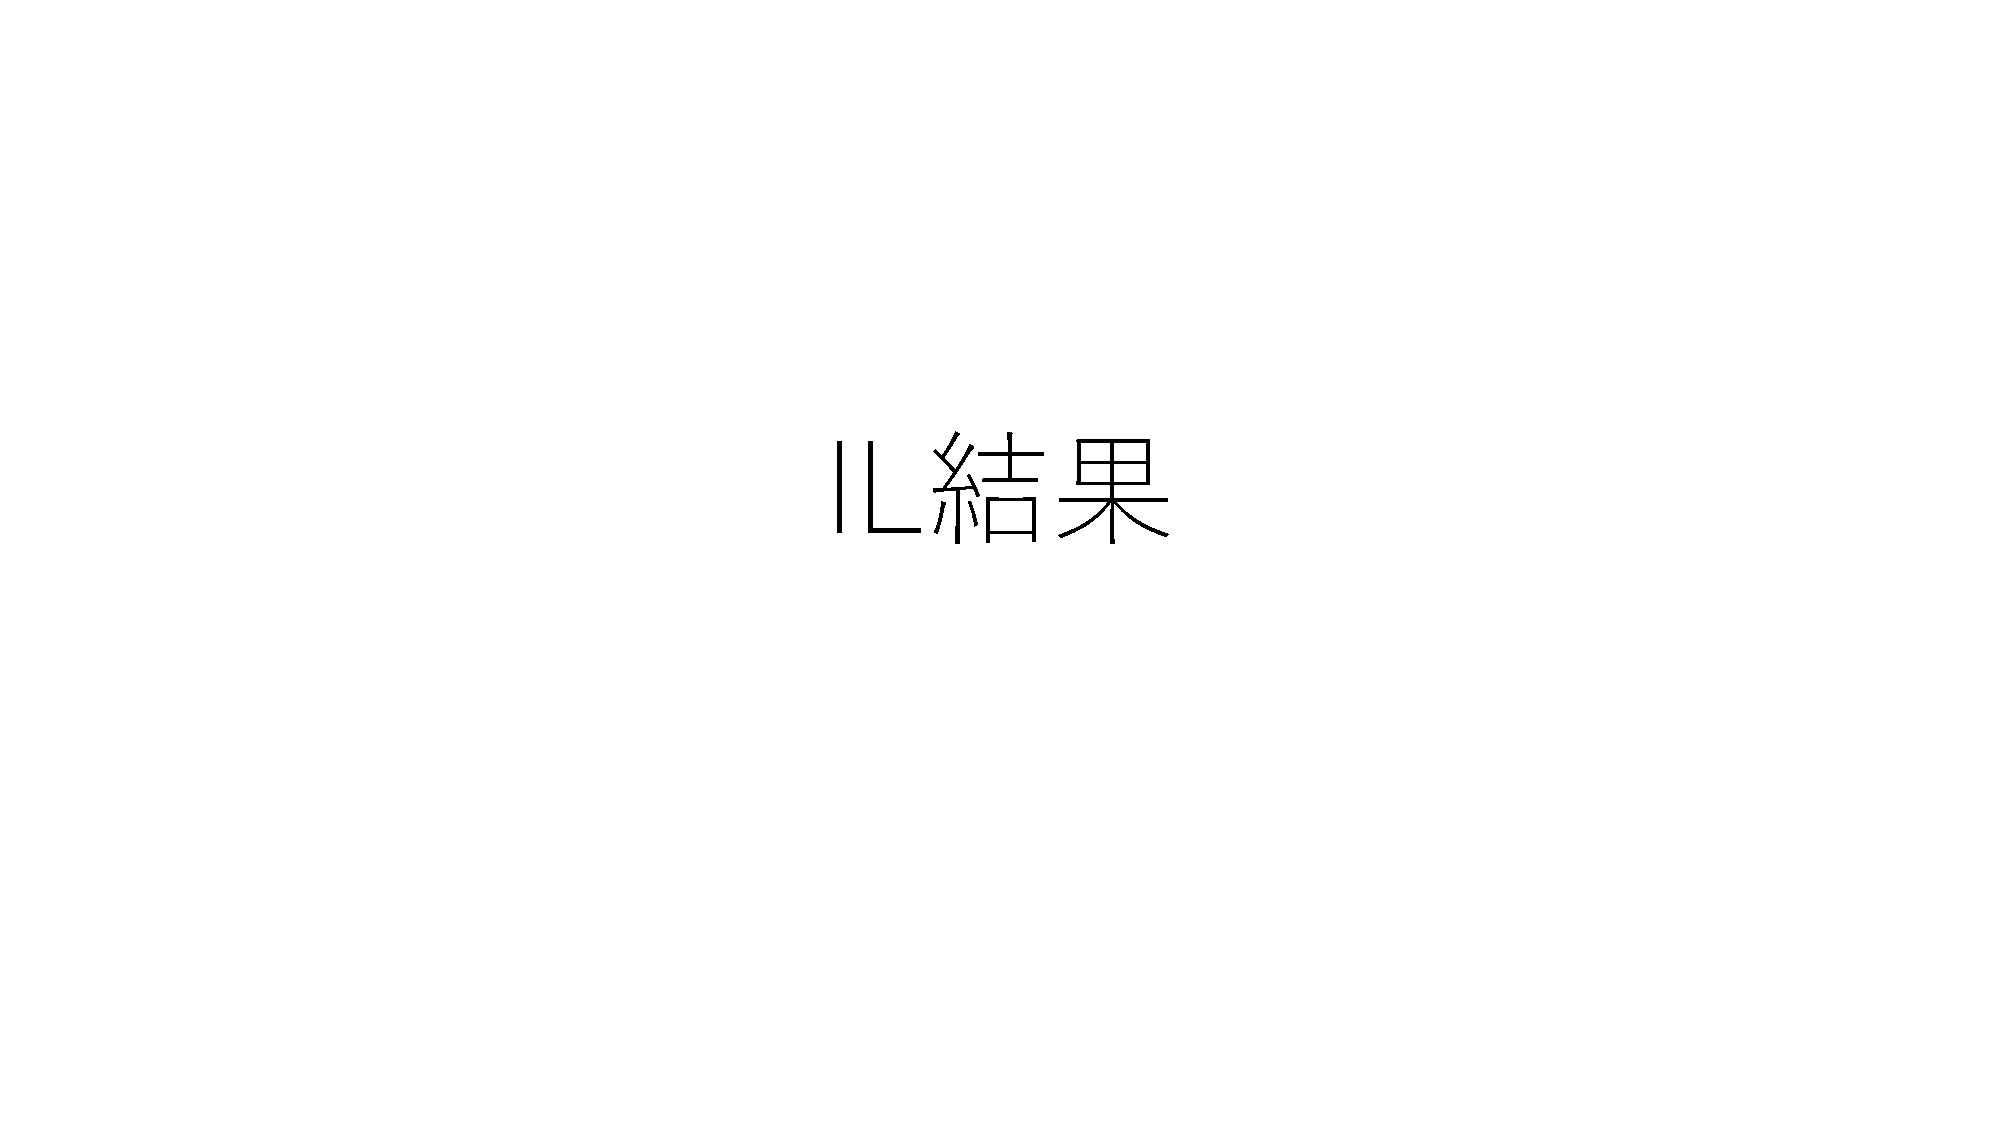
\includegraphics[width=15cm]{figure/fig_IL_result.pdf}
	\caption{ILの結果}
	\label{fig:IL_result}
\end{figure}
\subsection{内部量子効率と吸収係数の計算}
\begin{figure}[htbp]
	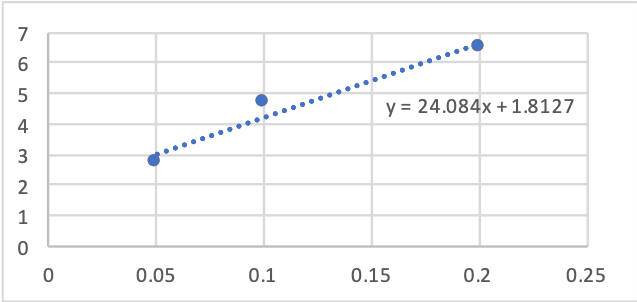
\includegraphics[width=15cm]{figure/fig_efficientcy_vs_L_inverce.png}
	\caption{外部量子効率 対共振器長の逆数}
	\label{fig:efficientcy_vs_L_inverce}
\end{figure}
\subsection{電流広がりに関する考察}
\section{電流注入利得スイッチング}
\subsection{3QW}
\subsection{10QW}
10周期量子井戸リッジ導波路型レーザーに関して電流注入利得スイッチング実験を行った。その結果を示す。


